\documentclass[a4paper, 12pt]{article}

\usepackage{fontspec}
\usepackage{polyglossia}
\defaultfontfeatures{Ligatures=TeX}
\setdefaultlanguage{russian}
\setotherlanguage{english}
\setmainfont{Times New Roman}
\newfontfamily{\latinfont}{Times New Roman}
\newfontfamily{\cyrillicfont}{Times New Roman}
\newfontfamily{\cyrillicfonttt}{Courier New}

\usepackage{geometry}
\usepackage{amsmath}
\usepackage{amssymb}
\usepackage{amsfonts}
\usepackage{graphicx}
\usepackage{float}
\usepackage{wrapfig}
\usepackage{subcaption}
%\usepackage[caption=false]{subfig}
\geometry{right=20mm}
\geometry{left=20mm}
\geometry{top=20mm}
\geometry{bottom=20mm}

\usepackage{indentfirst}
\usepackage[outputdir=auxiliary]{minted}

\graphicspath{{../img/}}
\DeclareMathOperator{\R}{\mathbb{R}}
\DeclareMathOperator{\C}{\mathbb{C}}
\renewcommand{\Re}{\mathrm{Re}}
\renewcommand{\Im}{\mathrm{Im}}


\DeclareMathOperator{\sign}{sgn}

\begin{document}
    \begin{titlepage}
    \begin{center}
        \textit{МИНИСТЕРСТВО ОБРАЗОВАНИЯ И НАУКИ\\
        РОССИЙСКОЙ ФЕДЕРАЦИИ}
        \vspace{1ex}

        федеральное государственное бюджетное образовательное учреждение\\
        высшего профессионального образования
        \vspace{1ex}

        \textbf{САНКТ-ПЕТЕРБУРГСКИЙ НАЦИОНАЛЬНЫЙ ИССЛЕДОВАТЕЛЬСКИЙ УНИВЕРСИТЕТ ИТМО}
        \vspace{13ex}

        Лабораторная работа №3\\
        <<Динамика нелинейных систем>>\\
        по дисциплине <<Моделирование технических систем>>\\
        \vspace{1em}
        Вариант 3\\
    \end{center}
    \vspace{14em}
    \begin{flushright}
        \noindent
        Выполнили:\\
        студенты гр. R4133c\\
        Борисов М. В.\\
        Симонов П.\\
        Мацуганов А. И.\\
        \vspace{1em}
        Преподаватель:\\
        Семенов Д. М.
    \end{flushright}
    \vfill
    \begin{center}
        \large{Санкт-Петербург}\\
        2021 г.\\
    \end{center}
\end{titlepage}

    \setcounter{page}{2}
    \setlength{\parindent}{0pt}

    \section*{Задание 1}
    Дана система с задержкой
    \begin{equation}
        \label{z1_sys}
        \dot{x}(t) = -\sign x(t-h),\ t \geq 0,\ h>0
    \end{equation}
    $h = 2$ - постоянная задержка, $x(t) = \varphi(t)$ при $t\in \left[ -h, 0 \right]$

    \begin{equation*}
        \varphi(t) =
        \left\{
        \begin{aligned}
            &0.5, &t& \in \left[ -2, -1 \right),\\
            &-t - 0.5, &t& \in \left[ -1, 0 \right].
        \end{aligned}
        \right.
    \end{equation*}

    Используя метод шагов, построить график решения системы~\eqref{z1_sys}.

    \subsection*{Решение}
    \begin{figure}[H]
        \centering
        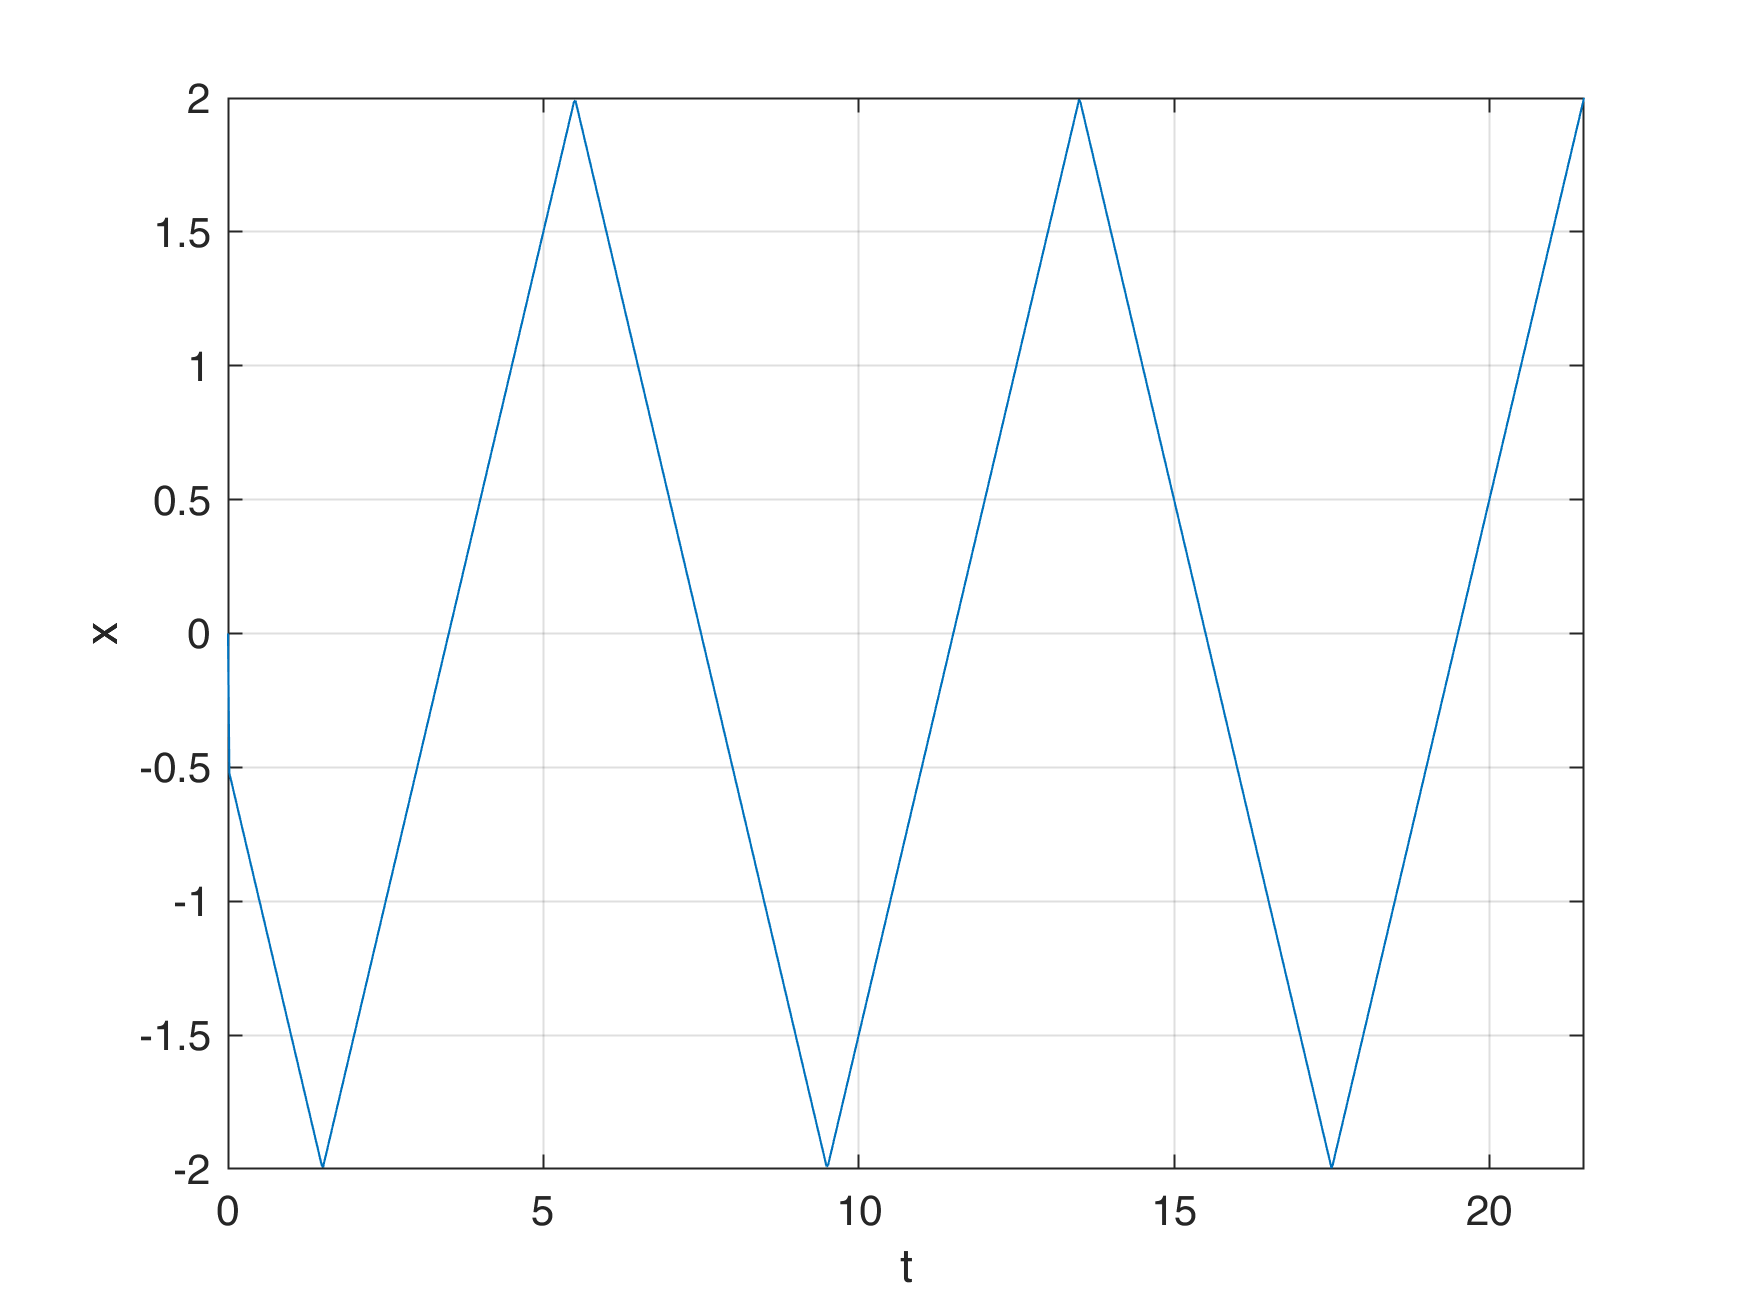
\includegraphics[width=0.75\linewidth]{Z1.png}
        \caption{График решения системы после трёх шагов}
    \end{figure}
    \paragraph*{Шаг 1} $t \in \left[ 0,\,2 \right]$
    \\
    \\$x(0) = \varphi(0) = -0.5 $
    \begin{equation}
        \dot{x} =
        \left\{
        \begin{aligned}
            -1,\,t \in \left( 0,\,1.5 \right]\\
            1,\,t \in \left( 1.5,\,2 \right]
        \end{aligned}
        \right.
    \end{equation}

    $t \in \left( 0,\,1.5 \right]$
    \begin{equation}
        x(t) = -t + C = \left| C = x(0) + 0 = -0.5\right| = -t - 0.5
    \end{equation}

    $t \in \left( 1.5,\,2 \right]$
    \begin{equation}
        x(t) = t + C = \left| C = x(1.5) - 1.5 = -3.5\right| = t - 3.5
    \end{equation}

    \paragraph*{Шаг 2} $t \in \left[ 2,\,4 \right]$
    \\
    \begin{equation}
        \dot{x} = 1,\,t \in \left( 2,\,4 \right]
    \end{equation}

    $t \in \left( 2,\,4 \right]$
    \begin{equation}
        x(t) = t + C = \left| C = x(2) - 2 = -3.5\right| = -t - 3.5
    \end{equation}

    \paragraph*{Шаг 3} $t \in \left[ 4,\,6 \right]$
    \\
    \begin{equation}
        \dot{x} =
        \left\{
        \begin{aligned}
            1,\,t \in \left( 4,\,5.5 \right]\\
            -1,\,t \in \left( 5.5,\,6 \right]
        \end{aligned}
        \right.
    \end{equation}

    $t \in \left( 4,\,5.5 \right]$
    \begin{equation}
        x(t) = t + C = \left| C = x(4) - 4 = -3.5\right| = t - 3.5
    \end{equation}

    $t \in \left( 5.5,\,6 \right]$
    \begin{equation}
        x(t) = -t + C = \left| C = x(5.5) + 5.5 = 7.5\right| = -t + 7.5
    \end{equation}

    \section*{Задание 2}
    Дана система с некоторой произвольной задержкой $\tau(t)$:
    \begin{equation}
        \label{z2_sys}
        \dot{x}(t) = -2x(t) - 0.1x(t- \tau(t))
    \end{equation}

    \begin{enumerate}
        \item Построить функцию Ляпунова
        \item Методом Разумихина доказать устойчивость системы
    \end{enumerate}

    \subsection*{Решение}
    Согласно методу Разумихина, система~\eqref{z2_sys} является асимптотически устойчивой,
    когда разрешимо линейное матричное неравенство:

    \begin{equation}
        \psi =
        \begin{bmatrix}
            A^T P+PA+q\left(\varepsilon+1\right)P & PA_{1}\\
            A_{1}^T P & -qP
        \end{bmatrix}
        < 0,\,q>0,\,P>0
    \end{equation}

    Пусть $\varepsilon = \dfrac{1}{2}$, из~\eqref{z2_sys} следует, что $A = -2,\,A_1=-0.1$. Тогда имеем:

    \begin{equation}
        \psi =
        \begin{bmatrix}
            \dfrac{3Pq}{2}-4P & -\dfrac{P}{10}\\
            -\dfrac{P}{10} & -P\,q
        \end{bmatrix}
        < 0,\,q>0,\,P>0
    \end{equation}

    По критерию Сильвества получаем:
    \begin{equation}
        \left\{
        \begin{aligned}
            \dfrac{3\,P\,q}{2}-4\,P < 0\\
            -\dfrac{3\,P^2\,q^2}{2}+4\,P^2\,q-\dfrac{P^2}{100} > 0\\
            q>0,\,P>0
        \end{aligned}
        \right.
    \end{equation}
    \begin{equation}
        \left\{
        \begin{aligned}
            0 < q < 2.67\\
            0.0025 < q < 2.66\\
            q>0,\,P>0
        \end{aligned}
        \right.
    \end{equation}

    Таким образом неравенство разрешимо и $\forall q \in (0.0025,\,2.66) \therefore$ система асимптотически устойчива.

    \section*{Задание 3}
    Дана система с постоянной задержкой $h$
    \begin{equation}
        \label{z3_sys}
        \dot{x}(t) = Ax(t) + A_1 x(t- h), \, \mbox{где } x \in \R^2
    \end{equation}

    \begin{equation*}
        A =
        \begin{pmatrix}
            -4& 1\\
            -2& -4
        \end{pmatrix}
        ,\,A_1 =
        \begin{pmatrix}
            1& 2\\
            1& -1
        \end{pmatrix}
        ,\, h =3
    \end{equation*}

    \begin{enumerate}
        \item Промоделировать данную систему
        \item Доказать устойчивость системы с помощью функционала Ляпунова-Красовского
    \end{enumerate}

    \subsection*{Решение}
    \begin{figure}[H]
        \centering
        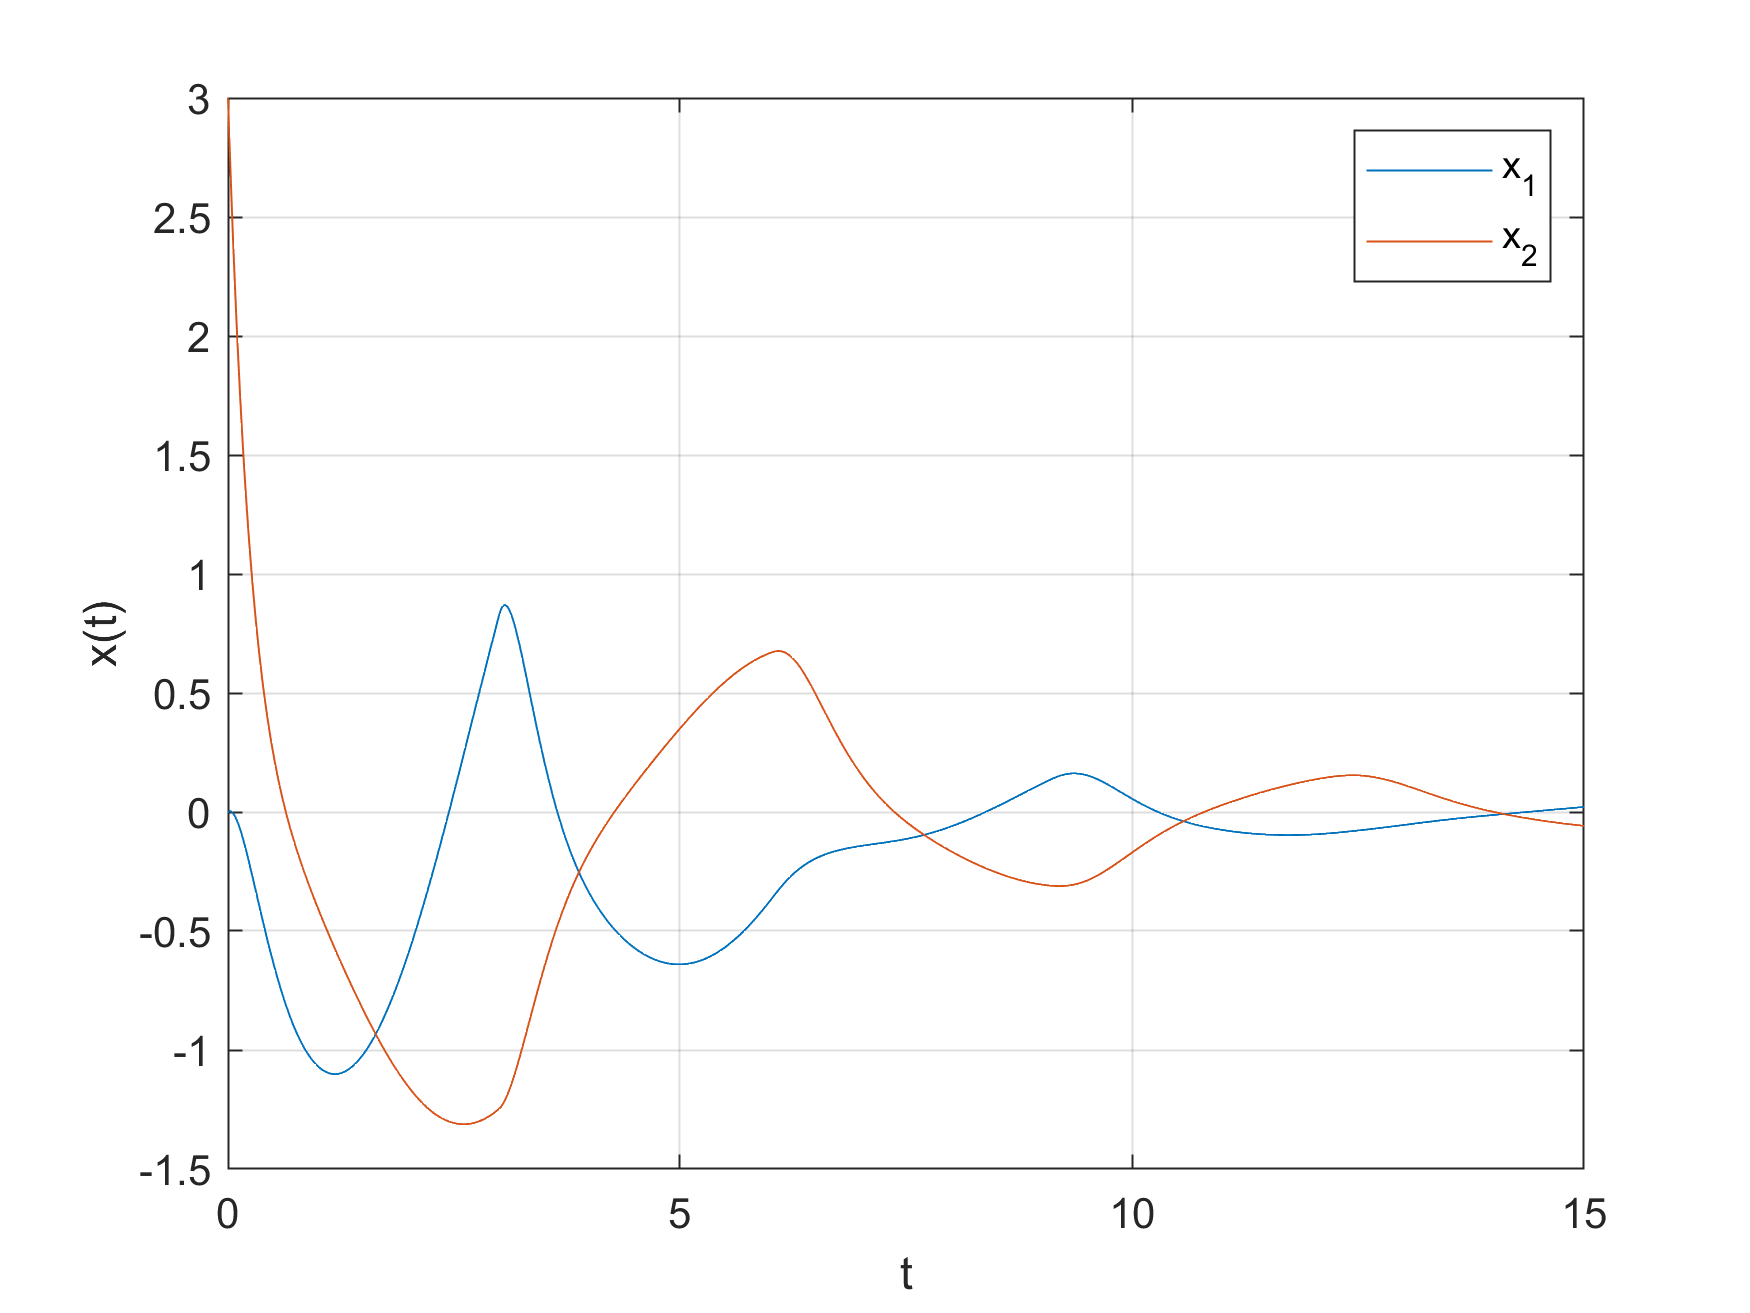
\includegraphics[width=0.75\linewidth]{Z3.png}
        \caption{Моделирование системы~\eqref{z3_sys} с задержкой $h=3$}
    \end{figure}

    Решая с помощью MATLAB матричное неравенство вида
    \begin{equation}
        \psi =
        \begin{bmatrix}
            A^T P + PA + Q & A_{1}^TP\\
            A_{1}^TP & -\left( 1-\dot{\tau} \right)Q
        \end{bmatrix}
        < 0,\,q>0,\,P>0
    \end{equation}
    получаем следующие значения:
    \begin{equation}
        P =
        \begin{bmatrix}
            0.3189 &  -0.0205\\
            -0.0205 &   0.3154
        \end{bmatrix}
        ,\,Q =
        \begin{bmatrix}
            1.0550 &   0.1088\\
            0.1088 &   1.2869
        \end{bmatrix}
    \end{equation}
    Решение найдено, значит система устойчива.

    \section*{Вывод}
    В данной работе были рассмотрены системы с запаздыванием и методы их исследования:
    \begin{itemize}
        \item Метод шагов для нахождения решения систем с запаздыванием
        \item Методы Разумихина и Ляпунова-Красовского для доказательства устойчивости систем с произвольной и постоянной задержкой соответственно
    \end{itemize}
\end{document}
